\chapter{Digital Logic: Combinational Circuits}

A processor is built out of transistors acting as switches. We abstract
transistors into \emph{logic gates}, gates into \emph{combinational
circuits} (whose outputs depend only on current inputs), and later add
memory to get \emph{sequential circuits}.

\section{Boolean Algebra}

Signals take one of two values, 0 (false, low voltage) and 1 (true, high
voltage). The basic operations are
\begin{itemize}
  \item AND: $A \cdot B$ (or $AB$), 1 iff both are 1;
  \item OR: $A + B$, 1 iff at least one is 1;
  \item NOT: $\overline{A}$ (or $A'$), flips the bit.
\end{itemize}
Derived operations: NAND $\overline{AB}$, NOR $\overline{A+B}$,
XOR $A \oplus B = A\overline{B} + \overline{A}B$, XNOR $\overline{A\oplus B}$.

\begin{center}
\begin{tabular}{cc|cccccc}
\toprule
$A$ & $B$ & AND & OR & NAND & NOR & XOR & XNOR \\
\midrule
0 & 0 & 0 & 0 & 1 & 1 & 0 & 1 \\
0 & 1 & 0 & 1 & 1 & 0 & 1 & 0 \\
1 & 0 & 0 & 1 & 1 & 0 & 1 & 0 \\
1 & 1 & 1 & 1 & 0 & 0 & 0 & 1 \\
\bottomrule
\end{tabular}
\end{center}

\subsection{Laws}

\begin{center}
\begin{tabular}{lll}
\toprule
Law & AND form & OR form \\
\midrule
Identity & $A\cdot 1 = A$ & $A + 0 = A$ \\
Null & $A \cdot 0 = 0$ & $A + 1 = 1$ \\
Idempotent & $AA = A$ & $A + A = A$ \\
Complement & $A\overline{A} = 0$ & $A + \overline{A} = 1$ \\
Commutative & $AB = BA$ & $A+B = B+A$ \\
Associative & $(AB)C = A(BC)$ & $(A+B)+C = A+(B+C)$ \\
Distributive & $A(B+C) = AB+AC$ & $A + BC = (A+B)(A+C)$ \\
Absorption & $A(A+B) = A$ & $A + AB = A$ \\
De Morgan & $\overline{AB} = \overline{A}+\overline{B}$ &
  $\overline{A+B} = \overline{A}\,\overline{B}$ \\
\bottomrule
\end{tabular}
\end{center}

Note the second distributive law $A + BC = (A+B)(A+C)$, which has no
analogue in ordinary arithmetic. Every law has a \emph{dual} obtained by
swapping AND/OR and 0/1.

\begin{example}
Simplify $F = \overline{A}B + AB + A\overline{B}$.
\[
F = (\overline{A}+A)B + A\overline{B} = B + A\overline{B}
  = (B + A)(B + \overline{B}) = A + B.
\]
\end{example}

\section{Gates}

\begin{figure}[H]
\centering
\begin{tikzpicture}[circuit logic US, every circuit symbol/.style={thick}]
  \node[and gate, inputs=nn] (a) at (0,0) {};
  \node[or gate, inputs=nn] (o) at (2.5,0) {};
  \node[not gate] (n) at (5,0) {};
  \node[nand gate, inputs=nn] (na) at (7,0) {};
  \node[xor gate, inputs=nn] (x) at (9.5,0) {};
  \node[below=4mm] at (a) {AND};
  \node[below=4mm] at (o) {OR};
  \node[below=4mm] at (n) {NOT};
  \node[below=4mm] at (na) {NAND};
  \node[below=4mm] at (x) {XOR};
\end{tikzpicture}
\caption{Standard (US) gate symbols. A bubble on an output means inversion.}
\end{figure}

\begin{important}[Universality]
NAND alone is \emph{functionally complete}: $\overline{A} = \overline{AA}$,
$AB = \overline{\overline{AB}}$, $A+B = \overline{\overline{A}\,\overline{B}}$.
The same is true for NOR. Real CMOS hardware prefers NAND/NOR because they
need fewer transistors than AND/OR.
\end{important}

\section{Truth Tables and Canonical Forms}

Any Boolean function of $n$ inputs is described by a truth table with $2^n$
rows.

\begin{definition}
A \textbf{minterm} is a product (AND) containing every variable once, either
plain or complemented; it is 1 in exactly one row. The \textbf{sum of
products (SOP)} form is the OR of the minterms for rows where $F = 1$.
Dually, a \textbf{maxterm} is a sum that is 0 in exactly one row, and the
\textbf{product of sums (POS)} form ANDs the maxterms of the rows where
$F = 0$.
\end{definition}

\begin{example}[Majority function]
$F(A,B,C) = 1$ iff at least two inputs are 1.
\begin{center}
\begin{tabular}{ccc|c}
\toprule
$A$ & $B$ & $C$ & $F$ \\
\midrule
0&0&0&0\\ 0&0&1&0\\ 0&1&0&0\\ 0&1&1&1\\
1&0&0&0\\ 1&0&1&1\\ 1&1&0&1\\ 1&1&1&1\\
\bottomrule
\end{tabular}
\end{center}
SOP: $F = \overline{A}BC + A\overline{B}C + AB\overline{C} + ABC
= \sum m(3,5,6,7)$. This simplifies to $F = AB + AC + BC$.
\end{example}

\section{Karnaugh Maps}

A K-map arranges the truth table in a grid whose rows and columns follow
\textbf{Gray code} order (00, 01, 11, 10) so that physically adjacent cells
differ in exactly one variable. Adjacent 1s can then be combined, since
$XY + X\overline{Y} = X$.

\textbf{Rules for grouping}:
\begin{enumerate}
  \item Groups must be rectangles of size $1, 2, 4, 8, \ldots$ (powers of 2).
  \item Groups may wrap around the edges (the map is a torus).
  \item Make groups as large as possible, and use as few as possible; every
    1 must be covered; overlapping is allowed.
  \item Don't-care entries (X) may be included in a group if that helps,
    but need not be covered.
\end{enumerate}
Each group of $2^k$ cells eliminates $k$ variables.

\begin{example}
Majority function K-map (rows $A$, columns $BC$):
\begin{center}
\begin{tabular}{c|cccc}
$A \backslash BC$ & 00 & 01 & 11 & 10 \\
\hline
0 & 0 & 0 & 1 & 0 \\
1 & 0 & 1 & 1 & 1 \\
\end{tabular}
\end{center}
Three groups of two: the column $BC = 11$ gives $BC$; cells $(1,01),(1,11)$
give $AC$; cells $(1,11),(1,10)$ give $AB$. So $F = AB + AC + BC$.

\begin{center}
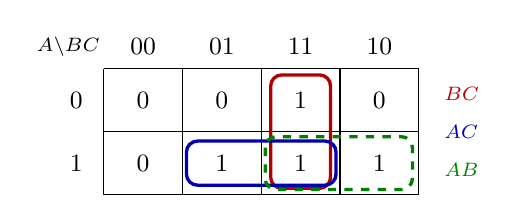
\begin{tikzpicture}[x=1cm, y=0.8cm, font=\small]
  \foreach \c/\lab in {0/00, 1/01, 2/11, 3/10} \node at (\c+0.5,0.35) {\lab};
  \foreach \r in {0,1} \node at (-0.35,-\r-0.5) {\r};
  \node at (-0.45,0.35) {\scriptsize $A\backslash BC$};
  \foreach \c in {0,...,4} \draw (\c,0) -- (\c,-2);
  \foreach \r in {0,1,2} \draw (0,-\r) -- (4,-\r);
  \foreach \r/\row in {0/{0,0,1,0}, 1/{0,1,1,1}} {
    \foreach \v [count=\c from 0] in \row \node at (\c+0.5,-\r-0.5) {\v};
  }
  \draw[very thick, red!70!black, rounded corners] (2.12,-0.1) rectangle (2.88,-1.9);
  \draw[very thick, blue!70!black, rounded corners] (1.05,-1.15) rectangle (2.95,-1.85);
  \draw[very thick, green!50!black, rounded corners, dashed] (2.05,-1.08) rectangle (3.92,-1.92);
  \node[red!70!black, font=\scriptsize, right] at (4.2,-0.4) {$BC$};
  \node[blue!70!black, font=\scriptsize, right] at (4.2,-1.0) {$AC$};
  \node[green!50!black, font=\scriptsize, right] at (4.2,-1.6) {$AB$};
\end{tikzpicture}
\end{center}
The three overlapping groups of the majority K-map; overlapping is allowed
because $X + X = X$.
\end{example}

\begin{example}[Four variables]
$F(A,B,C,D) = \sum m(0,2,5,7,8,10,13,15)$.
\begin{center}
\begin{tabular}{c|cccc}
$AB \backslash CD$ & 00 & 01 & 11 & 10 \\
\hline
00 & 1 & 0 & 0 & 1 \\
01 & 0 & 1 & 1 & 0 \\
11 & 0 & 1 & 1 & 0 \\
10 & 1 & 0 & 0 & 1 \\
\end{tabular}
\end{center}
The four corners form one group (wrap-around) giving $\overline{B}\,\overline{D}$;
the middle $2\times 2$ block gives $BD$. Hence
$F = \overline{B}\,\overline{D} + BD = \overline{B \oplus D}$.

\begin{center}
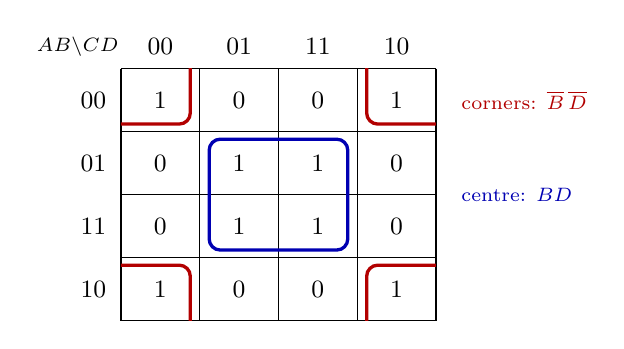
\begin{tikzpicture}[x=1cm, y=0.8cm, font=\small]
  \foreach \c/\lab in {0/00, 1/01, 2/11, 3/10} \node at (\c+0.5,0.35) {\lab};
  \foreach \r/\lab in {0/00, 1/01, 2/11, 3/10} \node at (-0.35,-\r-0.5) {\lab};
  \node at (-0.55,0.35) {\scriptsize $AB\backslash CD$};
  \foreach \r/\row in {0/{1,0,0,1}, 1/{0,1,1,0}, 2/{0,1,1,0}, 3/{1,0,0,1}} {
    \foreach \v [count=\c from 0] in \row \node at (\c+0.5,-\r-0.5) {\v};
  }
  \foreach \c in {0,...,4} \draw (\c,0) -- (\c,-4);
  \foreach \r in {0,...,4} \draw (0,-\r) -- (4,-\r);
  \begin{scope}
    \clip (0,0) rectangle (4,-4);
    \foreach \x/\y in {0/0, 4/0, 0/-4, 4/-4}
      \draw[very thick, red!70!black, rounded corners] (\x-0.88,\y+0.88) rectangle (\x+0.88,\y-0.88);
  \end{scope}
  \draw[very thick, blue!70!black, rounded corners] (1.12,-1.12) rectangle (2.88,-2.88);
  \node[red!70!black, font=\scriptsize, right] at (4.2,-0.5) {corners: $\overline{B}\,\overline{D}$};
  \node[blue!70!black, font=\scriptsize, right] at (4.2,-2) {centre: $BD$};
\end{tikzpicture}
\end{center}
The red group wraps around both edges: the map is really a torus, so the
four corners are mutually adjacent.
\end{example}

\section{Combinational Building Blocks}

\subsection{Multiplexer}

A \textbf{multiplexer (mux)} selects one of several inputs using select
lines. A 2-to-1 mux with inputs $I_0, I_1$ and select $S$:
\[ Y = \overline{S} I_0 + S I_1. \]
A $2^k$-to-1 mux needs $k$ select bits. Muxes are everywhere in the
datapath: whenever a value may come from two places, a mux chooses.

\begin{figure}[H]
\centering
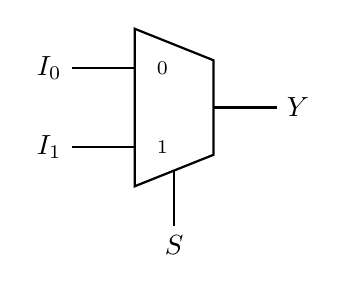
\begin{tikzpicture}[thick]
  \draw (0,0) -- (0,2) -- (1,1.6) -- (1,0.4) -- cycle;
  \draw (-0.8,1.5) node[left]{$I_0$} -- (0,1.5);
  \draw (-0.8,0.5) node[left]{$I_1$} -- (0,0.5);
  \draw (1,1) -- (1.8,1) node[right]{$Y$};
  \draw (0.5,0.2) -- (0.5,-0.5) node[below]{$S$};
  \node at (0.35,1.5) {\scriptsize 0};
  \node at (0.35,0.5) {\scriptsize 1};
\end{tikzpicture}
\caption{2-to-1 multiplexer.}
\end{figure}

A mux of $n$-bit buses is just $n$ one-bit muxes sharing the select line.

\subsection{Decoder}

An $n$-to-$2^n$ \textbf{decoder} has $n$ inputs and $2^n$ outputs; exactly
the output whose index equals the input value is 1. A 2-to-4 decoder:
$Y_0 = \overline{A_1}\,\overline{A_0}$, $Y_1 = \overline{A_1}A_0$,
$Y_2 = A_1\overline{A_0}$, $Y_3 = A_1A_0$. Decoders select a register
in the register file and a row in memory. An \textbf{encoder} does the
reverse.

\subsection{Adders}

\begin{definition}
A \textbf{half adder} adds two bits: $S = A \oplus B$, $C_{out} = AB$.
A \textbf{full adder} also takes a carry-in:
\[
S = A \oplus B \oplus C_{in}, \qquad
C_{out} = AB + AC_{in} + BC_{in}.
\]
\end{definition}

\begin{center}
\begin{tabular}{ccc|cc}
\toprule
$A$ & $B$ & $C_{in}$ & $C_{out}$ & $S$ \\
\midrule
0&0&0&0&0\\ 0&0&1&0&1\\ 0&1&0&0&1\\ 0&1&1&1&0\\
1&0&0&0&1\\ 1&0&1&1&0\\ 1&1&0&1&0\\ 1&1&1&1&1\\
\bottomrule
\end{tabular}
\end{center}

Notice $C_{out}$ is exactly the majority function.

\begin{figure}[H]
\centering
\begin{tikzpicture}[circuit logic US, huge circuit symbols, every circuit symbol/.style={thick}, thick]
  \node[xor gate, inputs=nn] (x1) at (2,1.2) {};
  \node[xor gate, inputs=nn] (x2) at (5.4,0.85) {};
  \node[and gate, inputs=nn] (a1) at (5.4,-0.6) {};
  \node[and gate, inputs=nn] (a2) at (5.4,-2) {};
  \node[or gate, inputs=nn] (o1) at (7.5,-1.3) {};
  % inputs
  \draw (-0.6,2.0) node[left]{$A$} -- (1.0,2.0) |- (x1.input 1);
  \draw (-0.6,0 |- x1.input 2) node[left]{$B$} -- (x1.input 2);
  \fill (0.0,2.0) circle (1.5pt);
  \draw (0.0,2.0) |- (a2.input 1);
  \fill (0.4,0 |- x1.input 2) circle (1.5pt);
  \draw (0.4,0 |- x1.input 2) |- (a2.input 2);
  \path (x2.input 2) ++(-0.4,0) coordinate (cu);
  \path (x2.input 2) ++(-0.9,0) coordinate (cb);
  \draw (-0.6,0.2) node[left]{$C_{in}$} -- (cu |- 0,0.2) -- (cu) -- (x2.input 2);
  \fill (cb |- 0,0.2) circle (1.5pt);
  \draw (cb |- 0,0.2) |- (a1.input 1);
  % A xor B to second xor and to the lower AND input
  \draw (x1.output) -- ++(0.5,0) coordinate(j) |- (x2.input 1);
  \draw (j) |- (a1.input 2);
  \fill (j) circle (1.5pt);
  % outputs
  \draw (x2.output) -- ++(2.4,0) node[right]{$S$};
  \draw (a1.output) -- ++(0.4,0) |- (o1.input 1);
  \draw (a2.output) -- ++(0.4,0) |- (o1.input 2);
  \draw (o1.output) -- ++(0.6,0) node[right]{$C_{out}$};
\end{tikzpicture}
\caption{A full adder from two half adders: $S = (A\oplus B)\oplus C_{in}$
and $C_{out} = AB + C_{in}(A\oplus B)$, which equals the majority function.}
\end{figure}

\paragraph{Ripple-carry adder.} Chain $n$ full adders, the carry-out of bit
$i$ feeding the carry-in of bit $i+1$. Simple, but the delay is $\Theta(n)$
because the carry may have to ripple through every stage.

\begin{figure}[H]
\centering
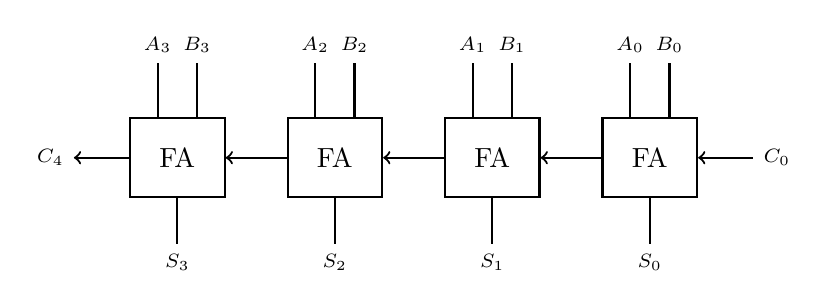
\begin{tikzpicture}[thick, box/.style={draw, minimum width=1.2cm, minimum height=1cm}]
  \foreach \i/\x in {3/0,2/2,1/4,0/6} {
    \node[box] (fa\i) at (\x,0) {FA};
    \draw (\x-0.25,1.2) node[above]{\scriptsize $A_\i$} -- (\x-0.25,0.5);
    \draw (\x+0.25,1.2) node[above]{\scriptsize $B_\i$} -- (\x+0.25,0.5);
    \draw (\x,-0.5) -- (\x,-1.1) node[below]{\scriptsize $S_\i$};
  }
  \draw[->] (fa0.west) -- (fa1.east);
  \draw[->] (fa1.west) -- (fa2.east);
  \draw[->] (fa2.west) -- (fa3.east);
  \draw[<-] (fa0.east) -- ++(0.7,0) node[right]{\scriptsize $C_0$};
  \draw[->] (fa3.west) -- ++(-0.7,0) node[left]{\scriptsize $C_4$};
\end{tikzpicture}
\caption{4-bit ripple-carry adder.}
\end{figure}

\paragraph{Carry-lookahead (idea).} Define \emph{generate} $g_i = A_iB_i$
and \emph{propagate} $p_i = A_i + B_i$. Then $c_{i+1} = g_i + p_ic_i$, which
can be expanded, e.g.\ $c_2 = g_1 + p_1g_0 + p_1p_0c_0$, so all carries are
computed in parallel in a constant number of gate levels (at the cost of
more gates). Hierarchical lookahead gives $\Theta(\log n)$ delay.

\paragraph{Subtraction.} $A - B = A + \overline{B} + 1$ in two's complement:
invert $B$ with XOR gates and set $C_0 = 1$. A single control bit
(\code{Binvert}) turns an adder into an adder/subtractor.

\subsection{The ALU}

The \textbf{arithmetic logic unit} computes one of several operations on two
32-bit inputs, chosen by a control input. A 1-bit ALU slice contains an AND
gate, an OR gate and a full adder, with a mux choosing the result;
32 slices are chained through the carries.

\begin{figure}[H]
\centering
\begin{tikzpicture}[circuit logic US, large circuit symbols, every circuit symbol/.style={thick}, thick, >=Stealth, font=\small]
  % gates
  \node[and gate, inputs=nn] (and) at (4,1.6) {};
  \node[or gate, inputs=nn] (or) at (4,0.4) {};
  \node[draw, minimum width=0.9cm, minimum height=1.1cm] (fa) at (4,-1.6) {$+$};
  % Binvert mux
  \draw (1.4,-0.6) -- (1.4,-2) -- (1.9,-1.8) -- (1.9,-0.8) -- cycle;
  \node[font=\tiny] at (1.55,-0.95) {0}; \node[font=\tiny] at (1.55,-1.65) {1};
  \node[not gate] (inv) at (0.55,-1.65) {};
  \draw (-0.6,-0.95) node[left]{$b$} -- (1.4,-0.95);
  \fill (-0.2,-0.95) circle (1.5pt);
  \draw (-0.2,-0.95) |- (inv.input);
  \draw (inv.output) -- (1.4,-1.65);
  \draw (1.65,-1.9) -- (1.65,-2.6) node[below, font=\scriptsize]{Binvert};
  % a bus
  \draw (-0.6,2.2) node[left]{$a$} -- (2.4,2.2) -- (2.4,-1.35);
  \foreach \y in {1.6,0.4} \fill (2.4,\y+0.2) circle (0pt);
  \draw (2.4,0 |- and.input 1) -- (and.input 1);
  \draw (2.4,0 |- or.input 1) -- (or.input 1);
  \draw (2.4,-1.35) -- ($(fa.west)+(0,0.25)$);
  \fill (2.4,0 |- and.input 1) circle (1.5pt);
  \fill (2.4,0 |- or.input 1) circle (1.5pt);
  % b bus
  \draw (1.9,-1.3) -- (2.9,-1.3);
  \draw (2.9,-1.85) -- (2.9,0 |- and.input 2) -- (and.input 2);
  \draw (2.9,0 |- or.input 2) -- (or.input 2);
  \draw (2.9,-1.85) -- ($(fa.west)+(0,-0.25)$);
  \fill (2.9,-1.3) circle (1.5pt);
  \fill (2.9,0 |- or.input 2) circle (1.5pt);
  % operation mux
  \draw (5.6,2.3) -- (5.6,-2.3) -- (6.2,-1.7) -- (6.2,1.7) -- cycle;
  \node[font=\tiny] at (5.75,1.6) {0}; \node[font=\tiny] at (5.75,0.4) {1};
  \node[font=\tiny] at (5.75,-1.6) {2};
  \draw (and.output) -- (5.6,1.6);
  \draw (or.output) -- (5.6,0.4);
  \draw (fa.east) -- (5.6,-1.6);
  \draw (6.2,0) -- (6.8,0) node[right]{Result};
  \draw (5.9,2) -- (5.9,2.7) node[above, font=\scriptsize]{Operation};
  % carries
  \draw[<-] (fa.north) -- ++(0,0.5) node[above, font=\scriptsize]{CarryIn};
  \draw[->] (fa.south) -- ++(0,-0.6) node[below, font=\scriptsize]{CarryOut};
\end{tikzpicture}
\caption{One 1-bit ALU slice: AND, OR and a full adder compute in
parallel and the \code{Operation} mux picks one. \code{Binvert} selects
$\overline{b}$ for subtraction.}
\end{figure}

\begin{center}
\begin{tabular}{cl}
\toprule
ALU control & Function \\
\midrule
0000 & AND \\
0001 & OR \\
0010 & add \\
0110 & subtract \\
0111 & set on less than \\
1100 & NOR \\
\bottomrule
\end{tabular}
\end{center}
The 4-bit control is \code{Ainvert}, \code{Bnegate} (= \code{Binvert} and
$C_0$), and a 2-bit operation select. Extra outputs:
\begin{itemize}
  \item \textbf{Zero}: 1 if the result is 0 (NOR of all result bits); used
    by \code{beq} (subtract and test Zero).
  \item \textbf{Overflow}: for signed add, $C_{n} \oplus C_{n-1}$ (carry into
    the sign bit differs from carry out).
  \item \textbf{Set on less than}: compute $A - B$; the sign bit of the
    result (corrected for overflow) is routed to bit 0 of the output, all
    other bits 0.
\end{itemize}

\begin{figure}[H]
\centering
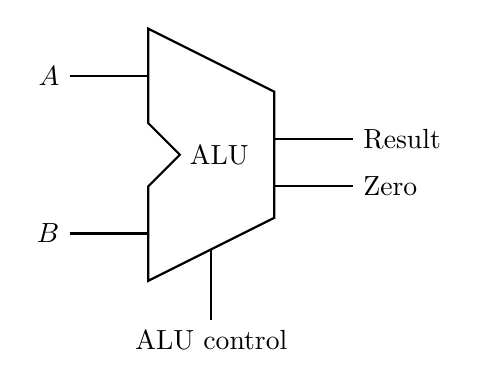
\begin{tikzpicture}[thick]
  \draw (0,0) -- (0,1.2) -- (0.4,1.6) -- (0,2) -- (0,3.2) -- (1.6,2.4) -- (1.6,0.8) -- cycle;
  \node at (0.9,1.6) {ALU};
  \draw (-1,2.6) node[left]{$A$} -- (0,2.6);
  \draw (-1,0.6) node[left]{$B$} -- (0,0.6);
  \draw (1.6,1.8) -- (2.6,1.8) node[right]{Result};
  \draw (1.6,1.2) -- (2.6,1.2) node[right]{Zero};
  \draw (0.8,-0.5) node[below]{ALU control} -- (0.8,0.4);
\end{tikzpicture}
\caption{ALU symbol.}
\end{figure}

\section{Timing}

Gates have \emph{propagation delay}. The delay of a combinational circuit is
the delay along its \textbf{critical path} (longest path from any input to
any output). This will determine the clock period of the processor.

\section*{Summary}
\begin{itemize}
  \item Boolean algebra laws (especially De Morgan) let us manipulate
    expressions; NAND and NOR are universal.
  \item Truth table $\to$ SOP via minterms $\to$ simplify with K-maps
    (Gray code, power-of-two groups, wrap-around, don't cares).
  \item Building blocks: mux (select), decoder (one-hot), full adder,
    ripple-carry and carry-lookahead adders, ALU with Zero and Overflow.
  \item Subtraction = add the complement plus 1.
\end{itemize}
